\documentclass[]{tufte-handout}

% ams
\usepackage{amssymb,amsmath}

\usepackage{ifxetex,ifluatex}
\usepackage{fixltx2e} % provides \textsubscript
\ifnum 0\ifxetex 1\fi\ifluatex 1\fi=0 % if pdftex
  \usepackage[T1]{fontenc}
  \usepackage[utf8]{inputenc}
\else % if luatex or xelatex
  \makeatletter
  \@ifpackageloaded{fontspec}{}{\usepackage{fontspec}}
  \makeatother
  \defaultfontfeatures{Ligatures=TeX,Scale=MatchLowercase}
  \makeatletter
  \@ifpackageloaded{soul}{
     \renewcommand\allcapsspacing[1]{{\addfontfeature{LetterSpace=15}#1}}
     \renewcommand\smallcapsspacing[1]{{\addfontfeature{LetterSpace=10}#1}}
   }{}
  \makeatother

\fi

% graphix
\usepackage{graphicx}
\setkeys{Gin}{width=\linewidth,totalheight=\textheight,keepaspectratio}

% booktabs
\usepackage{booktabs}

% url
\usepackage{url}

% hyperref
\usepackage{hyperref}

% units.
\usepackage{units}


\setcounter{secnumdepth}{-1}

% citations

% pandoc syntax highlighting

% longtable

% multiplecol
\usepackage{multicol}

% strikeout
\usepackage[normalem]{ulem}

% morefloats
\usepackage{morefloats}


% tightlist macro required by pandoc >= 1.14
\providecommand{\tightlist}{%
  \setlength{\itemsep}{0pt}\setlength{\parskip}{0pt}}

% title / author / date
\date{}


\begin{document}





\thispagestyle{empty}

\noindent\LARGE \emph{Bravakis Property}\\
\noindent\Large \emph{Forest Management Plan}\\
\noindent\Large \emph{March 12, 2020}

\normalsize 

\begin{marginfigure}
\hspace{2pt}\newline\vspace{80pt}
\noindent \textit{\large Effective date of plan}  
\newline\indent April 1, 2020  
\end{marginfigure}

\begin{marginfigure}
\noindent \textit{\large Property}   
\newline\indent 81 acres and dwelling   
\newline\indent Worcester, VT  
\newline\indent SPAN 788-251-10063  
\newline\indent Mapping based on VMP photo(s)  
\newline\indent 144212, 148212  
\end{marginfigure}

\begin{marginfigure}
\noindent \textit{\large Owner}
\newline\indent Louis and Olivia Bravakis  
\newline\indent 624 Hampshire Hill Road
\indent 
\newline\indent Worcester, VT 05682  
\end{marginfigure}

\begin{marginfigure}
\noindent \textit{\large Prepared by} 
\newline\indent Neal F. Maker and John D. Foppert  
\newline\indent Pekin Branch Forestry  
\newline\indent 1324 West County Road  
\newline\indent Calais, VT 05648  
\newline\indent (802) 229-9757  
\vspace{100pt}\end{marginfigure}

\vspace{30pt} \indent This forest management plan is a blueprint for
responsible land stewardship. It is the result of a planning process
that incorporated an assessment of the history and current conditions on
the property, consideration of the various courses of future development
that the forest could follow, and discernment as to which outcomes best
suit the landowners' particular objectives.

\vspace{20pt} By signing below, I certify that I approve of---and agree
to manage my forestland according to---the following management plan. I
further certify that any of my forestland that is enrolled in Vermont's
Use Value Appraisal program is under active long-term forest management
in accordance with the state's minimum acceptable standards for forest
management. These standards include following Acceptable Management
Practices to maintain water quality on logging operations.

\vspace{22pt}

\noindent\rule{7.3cm}{0.4pt} \rule{.3cm}{0pt} \rule{3cm}{0.4pt}

\noindent Landowner \rule{6cm}{0pt} Date

\vspace{18pt}

\noindent\rule{7.3cm}{0.4pt} \rule{.3cm}{0pt} \rule{3cm}{0.4pt}

\noindent Landowner \rule{6cm}{0pt} Date

\vspace{18pt}

\noindent\rule{7.3cm}{0.4pt} \rule{.3cm}{0pt} \rule{3cm}{0.4pt}

\noindent Landowner \rule{6cm}{0pt} Date

\vspace{18pt}

\noindent\rule{7.3cm}{0.4pt} \rule{.3cm}{0pt} \rule{3cm}{0.4pt}

\noindent Landowner \rule{6cm}{0pt} Date

\begin{marginfigure}

{\centering 
\includegraphics[width=0.9\linewidth,height=0.9\textheight]{C:/Users/Neal/projects/cruise/logo-small-gray80} 

}

\end{marginfigure}

\vspace{35pt}

This forest management plan meets the standards promulgated by the
Vermont Department of Forests, Parks and Recreation as required for
eligibility in the Use Value Appraisal Program.

\vspace{22pt}

\noindent\rule{7.3cm}{0.4pt} \rule{.3cm}{0pt} \rule{3cm}{0.4pt}

\noindent County Forester \rule{5.3cm}{0pt} Date

\pagebreak

\section{Introduction}\label{introduction}

This plan covers the ten year period from 2020 to 2029. It lays out the
near- and medium-term actions that should guide the development of the
Bravakis Forest. It also qualifies the property for Use Value Appraisal
(UVA) and commensurate reduction in property taxes.\footnote{Further
  information about UVA and current valuations can be found at the
  Vermont Tax Department's website:
  \url{https://tax.vermont.gov/property-owners/current-use}.
  \vspace{20pt}} Owners participating in the Use Value Appraisal program
are obliged to manage their property according to the plan and to make
any reasonable investments for improvement that the plan
recommends.\footnote{UVA management plan standards are determined by the
  Department of Forests, Parks, \& Recreation and are available at
  \url{https://fpr.vermont.gov/forest/your_woods/use_value_appraisal} or
  through a County Forester.}

The plan is organized to reflect the forest decision making process. It
begins with a general overview of the property, then lays out the
landowner's management goals, before exploring the forest in detail and
discussing the actions that could be taken to help meet those goals. Its
recommendations were developed in accordance with the principles and
practices of scientifically sound forestry, as described in the relevant
management guidelines, textbooks and academic journals.

\section{Property Description}\label{property-description}

Some 70 percent of the 81 acre Bravakis property is productive
forestland that will be managed according to this plan. Its elevations
range from 1050 to 1390 feet above mean sea level. The property is
located on the eastern slope of Mount Worcester, in one of Central
Vermont's most important habitat blocks; which encompasses the Worcester
Range and acts as a major wildlife corridor, connecting the unbroken
forests of the Green Mountains to the Northeastern Highlands. Two
unnamed headwater streams converge on the property and flow east into
the North Branch of the Winooski River. It is the last property on the
town maintained section of Hampshire Hill Road in northern Worcester.
Property lines are mostly marked with old intermittent wire fences.
Soils, forest health, and other pertinent topics are discussed in the
individual stand area descriptions that follow.

\section{Principles, Goals \& Strategies For Forest
Management}\label{principles-goals-strategies-for-forest-management}

The following sections describe the chief principles and goals that
should guide forest management on the property; and outline the general
strategies that can be used to support them.

\begin{marginfigure}

{\centering 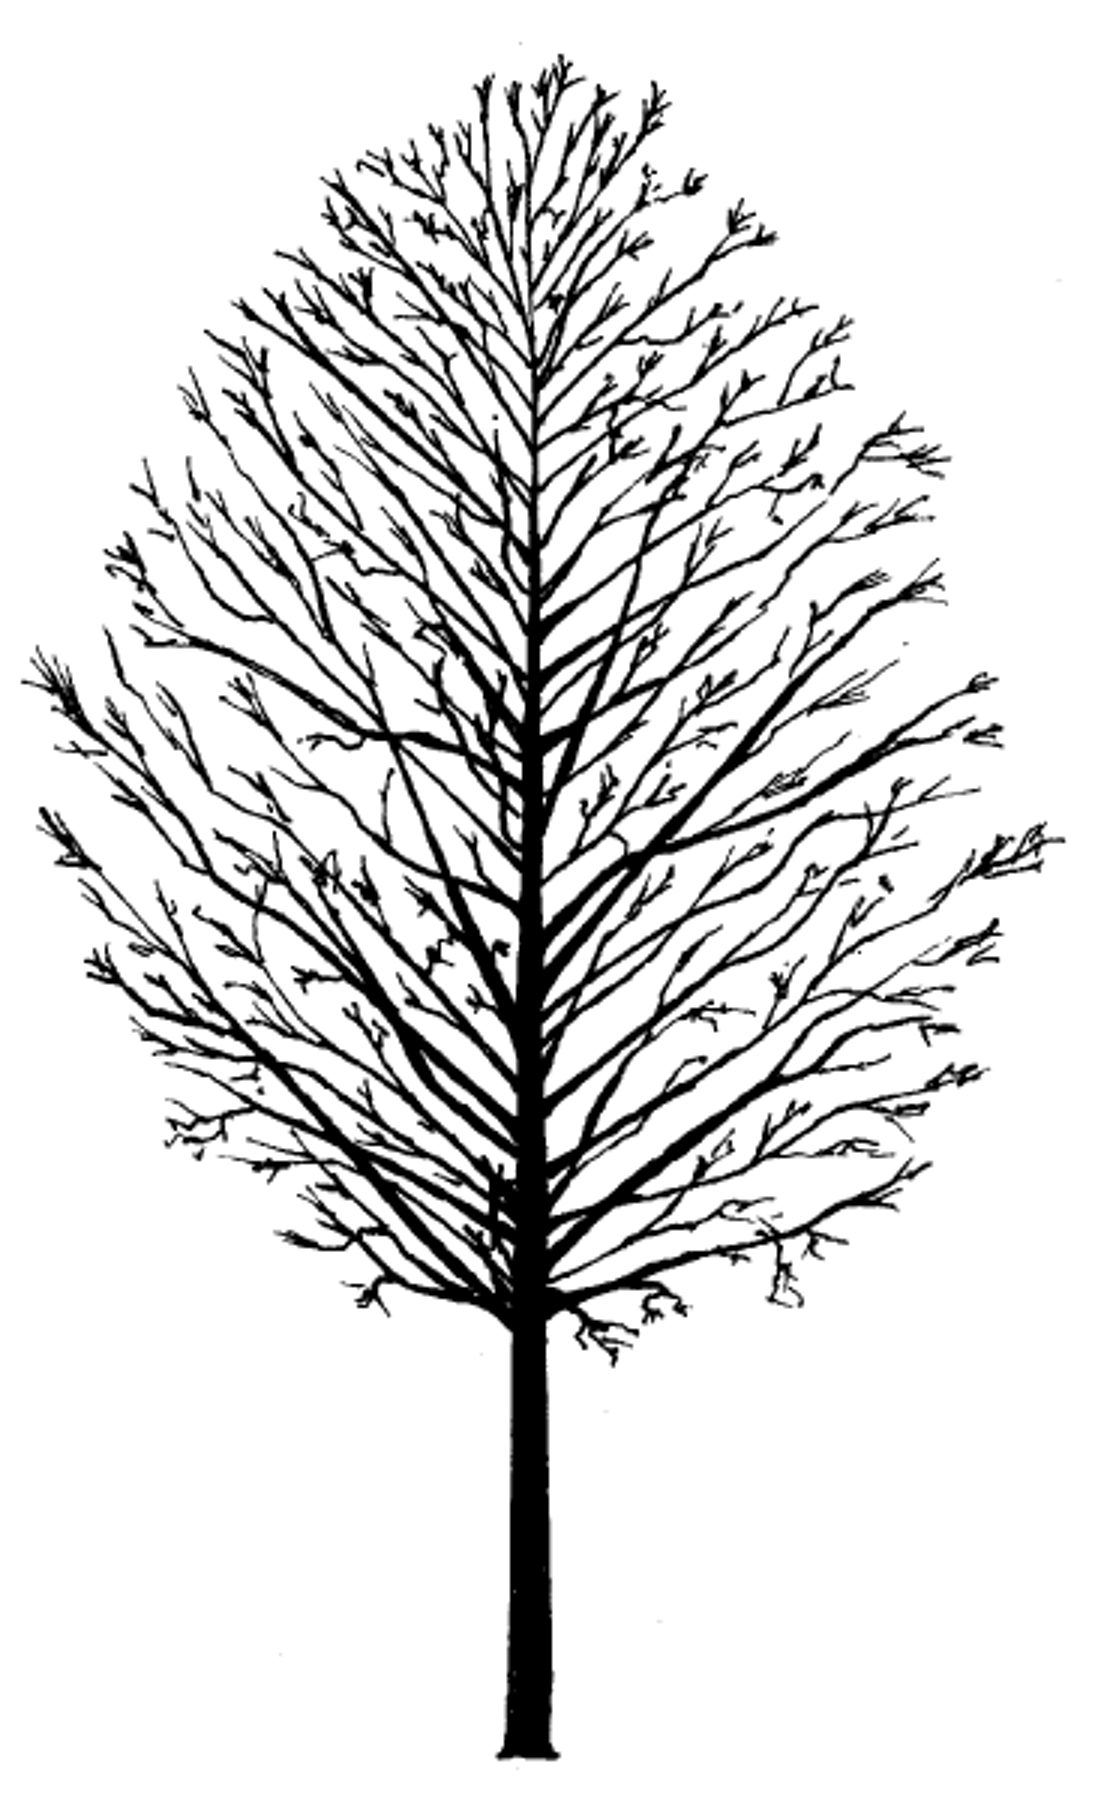
\includegraphics[width=0.7\linewidth,height=0.7\textheight]{C:/Users/Neal/projects/cruise/maple} 

}

\end{marginfigure}

\subsection{Conservation}\label{conservation}

The ecological functioning, productive capacity and biological diversity
of the forest resource should be maintained or improved over time so as
to provide opportunities for the current or future landowners to
continue to enjoy and use the property. A management strategy that is
sustainable in the long-term and viable in the short- and medium-terms
offers a strong measure of protection against future development or
conversion.

\subsection{Ecological integrity, wildlife habitat, and
biodiversity}\label{ecological-integrity-wildlife-habitat-and-biodiversity}

Management should prioritize the protection of critical ecological
functions, water resources, and threatened or rare plant and wildlife
communities. Wetlands and stream-side riparian zones should be carefully
delineated and protected; and management should give consideration to
the habitat needs of native wildlife populations and to the relationship
between the property, its neighbors and the larger landscape they are
nested within. Management should be informed by and aim to improve
landscape diversity, wildlife travel corridors, and habitat
connectivity. Locally under-represented habitat types should be
identified and promoted. Stand scale and sub-stand scale management
should focus on developing or maintaining species-specific habitat
needs, such as nesting sites, cover, mast production, preferred browse
or other unique structural and compositional requirements.

\subsection{Timber management}\label{timber-management}

Management should provide regular returns from timber harvesting.
Long-term value growth is provided by maintaining full site occupancy
with healthy trees capable of producing high quality sawtimber or
veneer. Tree species which yield sought-after, high-value wood should be
promoted within each stand or, when regenerating a new stand, attention
should be paid to creating stand conditions that favor the establishment
of those species. At a property-wide scale, a variety of species should
be maintained, providing options for seizing future market opportunities
and a hedge against species-specific market depreciation. Among desired
species, additional preference should be given to individual trees of
sufficient vigor and grade-potential for strong future value growth.
Consideration of economic efficiency should inform the timing and
coordination of infrastructure investments and stand maintenance,
improvement and harvest operations.

\section{Stand Descriptions \& Management
Recommendations}\label{stand-descriptions-management-recommendations}

\begin{marginfigure} \noindent \textit{\LARGE Management Schedule} 

 \vspace{10 pt} 

 \noindent \textit{\large 2023} 

 \begin{itemize} \item Area 5: Dominant-Tree Thinning 

 \end{itemize} \vspace{10 pt} 

 \noindent \textit{\large 2029} 

 \begin{itemize} \item Reinventory forest 

 \end{itemize} \end{marginfigure}

Presented below are detailed stand-by-stand descriptions of the forest,
the long-term structural, compositional and functional goals for each
stand, and the near-term silvicultural treatments or management
activities that have been prescribed to advance each stand toward those
goals. The data presented in the following pages was obtained from a
field examination of the property in February of 2020. General
conditions were assessed qualitatively in conjunction with quantitative
sampling. Observational notes and sample summary statistics together
provide the basis for the area descriptions and management
recommendations. All sampling was done using a systematic sample and
variable radius plots. In stands with uneven-aged structures, all trees
6" dbh and larger were measured in each plot. In stands with even-aged
structures, all main-canopy trees were measured in each plot.

When contractors are used to implement silvicultural prescriptions, they
should be highly skilled, properly equipped, fully insured, and closely
supervised. A professional forester should prepare and administer
commercial treatments, and logging operations should be timed to
coincide with favorable weather conditions (working on wet soils only
when they are frozen, for instance) and favorable timber markets. Use
Value Appraisal program guidelines allow any management activities
prescribed in this plan to be carried out up to three years before or
after the date indicated. Landowners in the Use Value Appraisal program
must file a Forest Management Activity Report with the County Forester
by February 1\textsuperscript{st} if any commercial logging occurred in
the previous year.

The property should be reinventoried in 2029 and the findings brought to
bear on a reassessment of the goals and strategies proposed in this
plan, leading to a formal management plan update. At any point over the
course of this management period, this plan may be updated to
incorporate new information and to reflect any new thoughts, concerns or
considerations on the part of the landowner or the foresters helping to
manage the land.

\newpage

\section{Area 1}\label{area-1}

Mixedwood\\
\noindent 11.23 legal acres \textbar{} 11.78 measured acres

\subsection{Site-specific information}\label{site-specific-information}

\begin{quote}
\begin{itemize}
\tightlist
\item
  \textbf{Soils:}\\
  \indent\indent  \textbf{Peru gravelly fine sandy loam} (deep,
  moderately well drained, dense glacial till on backslopes)
\end{itemize}
\end{quote}

\begin{quote}
\begin{itemize}
\tightlist
\item
  \textbf{Site Class:}\\
  \vspace{2pt} II (determined from soil mapping and field assessment)
\end{itemize}
\end{quote}

\begin{quote}
\begin{itemize}
\tightlist
\item
  \textbf{Access:}\\
  \vspace{2pt} Mostly easy to access from field. Less than one mile.
\end{itemize}
\end{quote}

\begin{quote}
\begin{itemize}
\tightlist
\item
  \textbf{Stand history:}\\
  \vspace{2pt} Old pasture abandoned 1940 or 1950. Poor quality trees
  were removed from the eastern section and chipped some 30 years ago,
  triggering the establishment of a second cohort (age-class) there.
\end{itemize}
\end{quote}

\subsection{Current forest
information}\label{current-forest-information}

\begin{quote}
\begin{itemize}
\tightlist
\item
  \textbf{Age Class Structure:}\\
  \vspace{2pt} Two-aged\\

  \begin{marginfigure}
  \includegraphics{fmp-vt_files/figure-latex/unnamed-chunk-2-1} \caption[Distributions are approximated with kernel density estimation]{Distributions are approximated with kernel density estimation. Common species are those that account for at least 8 percent of the total stocking and areas under each curve represent species basal areas.}\label{fig:unnamed-chunk-2}
  \end{marginfigure}
\end{itemize}
\end{quote}

\begin{quote}
\begin{itemize}
\tightlist
\item
  \textbf{Average stocking (with 95\% confidence intervals):}\\
  \vspace{2pt} 95 sq ft basal area (+/- 10 sq ft)\\
  9.4" quadratic stand diameter (+/- 1.9``)\\
  199 trees per acre (+/- 61 trees)\\
  \vspace{8pt}
\end{itemize}
\end{quote}

\begin{tabular}{lrrr}
\toprule
Size Class & Total & AGS & UGS\\
\midrule
6-11 in. & 55 & 55 & 0\\
12-15 in. & 35 & 30 & 5\\
16-21 in. & 5 & 5 & 0\\
22+ in. & 0 & 0 & 0\\
Total & 95 & 90 & 5\\
\bottomrule
\end{tabular}

\vspace{2pt}
\footnotesize\parbox{200pt}{Current basal area (sq ft/ac) of total growing stock, acceptable growing stock (AGS), and unacceptable growing stock (UGS) by size class.}\normalsize

\begin{quote}
\begin{itemize}
\tightlist
\item
  \textbf{Species (\% stocking):}\\
  \vspace{2pt} soft maple (58\%), spruce (32\%), fir (5\%), white pine
  (5\%)
\end{itemize}
\end{quote}

\begin{quote}
\begin{itemize}
\tightlist
\item
  \textbf{Regeneration:}\\
  \vspace{2pt} Soft maple and spruce regeneration throughout. Much stump
  sprouted soft maple in the northeast, where the logging occurred.
\end{itemize}
\end{quote}

\begin{quote}
\begin{itemize}
\tightlist
\item
  \textbf{Forest health:}\\
  \vspace{2pt} Good. No exotic invasives noted.
\end{itemize}
\end{quote}

\subsection{Inventory information}\label{inventory-information}

\begin{quote}
\begin{itemize}
\tightlist
\item
  2 points, 10 BAF, February, 2020
\end{itemize}
\end{quote}

\begin{figure}
\includegraphics{fmp-vt_files/figure-latex/unnamed-chunk-6-1} \caption[Points represent individual plots]{Points represent individual plots. Asterisk represnts stand average. Radial lines are quadratic stand diameters.}\label{fig:unnamed-chunk-6}
\end{figure}

\subsection{Long-term management
system}\label{long-term-management-system}

\textbf{Even-aged System}

The stand should generally be treated as even-aged, despite the second
cohort that has developed in the northeast. The stocking is lower in
that area, and young trees will have enough light to continue developing
until the overstory is eventually removed, in 30 years or so. We
generally expect a 100 year rotation length (the overstory is about 70
now) and thinnings every 10 or 15 years (perhaps once more before
regeneration). The southernmost corner of the stand is part of an area
the state has mapped as deer wintering habitat, which should be taken
into consideration when the time comes to regenerate. Also, an intact
canopy should be retained along the stream, to shade the water and
protect stream-side wildlife habitat; and some larger declining trees
and snags should be kept there, as den trees are especially important
near streams (DeGraaf et al.
\protect\hyperlink{ref-degraaf_technical_2006}{2006}).

\subsection{Silvicultural
prescription}\label{silvicultural-prescription}

No treatment is necessary in the next decade, as the stocking is already
near b-line.

\newpage

\section{Area 2}\label{area-2}

Mixedwood\\
\noindent 7.15 legal acres \textbar{} 7.50 measured acres

\subsection{Site-specific
information}\label{site-specific-information-1}

\begin{quote}
\begin{itemize}
\tightlist
\item
  \textbf{Soils:}\\
  \indent\indent  \textbf{Tunbridge-Lyman complex} (relatively deep to
  shallow, well drained to somewhat excessively drained, loose, very
  rocky glacial tills on backslopes, shoulders, and summits)\\
  \textbf{Peru gravelly fine sandy loam} (deep, moderately well drained,
  dense glacial till on backslopes)
\end{itemize}
\end{quote}

\begin{quote}
\begin{itemize}
\tightlist
\item
  \textbf{Site Class:}\\
  \vspace{2pt} II \& III (determined from soil mapping and field
  assessment)
\end{itemize}
\end{quote}

\begin{quote}
\begin{itemize}
\tightlist
\item
  \textbf{Access:}\\
  \vspace{2pt} Adjacent to field, but steep terrain limits movement
  somewhat in the east.
\end{itemize}
\end{quote}

\begin{quote}
\begin{itemize}
\tightlist
\item
  \textbf{Stand history:}\\
  \vspace{2pt} There is some age class structure in the stand, but the
  majority of trees look to date to the 1950s. The area may have been a
  ledgy, unimproved pasture, or it may have remained forested and had
  all the older trees cut out at some point. A bit of tending has been
  done recently.
\end{itemize}
\end{quote}

\subsection{Current forest
information}\label{current-forest-information-1}

\begin{quote}
\begin{itemize}
\tightlist
\item
  \textbf{Age Class Structure:}\\
  \vspace{2pt} Uneven-aged\\

  \begin{marginfigure}
  \includegraphics{fmp-vt_files/figure-latex/unnamed-chunk-7-1} \caption[Distributions are approximated with kernel density estimation]{Distributions are approximated with kernel density estimation. Common species are those that account for at least 8 percent of the total stocking and areas under each curve represent species basal areas.}\label{fig:unnamed-chunk-7}
  \end{marginfigure}
\end{itemize}
\end{quote}

\begin{quote}
\begin{itemize}
\tightlist
\item
  \textbf{Average stocking (with 95\% confidence intervals):}\\
  \vspace{2pt} 113 sq ft basal area (+/- 69 sq ft)\\
  9.3" quadratic stand diameter (+/- 1.3``)\\
  241 trees per acre (+/- 204 trees)\\
  \vspace{8pt}
\end{itemize}
\end{quote}

\begin{tabular}{lrrr}
\toprule
Size Class & Total & AGS & UGS\\
\midrule
6-11 in. & 77 & 57 & 20\\
12-15 in. & 30 & 20 & 10\\
16-21 in. & 7 & 7 & 0\\
22+ in. & 0 & 0 & 0\\
Total & 113 & 83 & 30\\
\bottomrule
\end{tabular}

\vspace{2pt}
\footnotesize\parbox{200pt}{Current basal area (sq ft/ac) of total growing stock, acceptable growing stock (AGS), and unacceptable growing stock (UGS) by size class.}\normalsize

\begin{quote}
\begin{itemize}
\tightlist
\item
  \textbf{Species (\% stocking):}\\
  \vspace{2pt} spruce (47\%), soft maple (15\%), beech (12\%), hard
  maple (9\%), yellow birch (9\%), ash (3\%), black cherry (3\%),
  hemlock (3\%)
\end{itemize}
\end{quote}

\begin{quote}
\begin{itemize}
\tightlist
\item
  \textbf{Regeneration:}\\
  \vspace{2pt} Very little. Widely scattered spruce, beech, and striped
  maple.
\end{itemize}
\end{quote}

\begin{quote}
\begin{itemize}
\tightlist
\item
  \textbf{Forest health:}\\
  \vspace{2pt} Mostly good. No exotic invasives noted.
\end{itemize}
\end{quote}

\subsection{Inventory information}\label{inventory-information-1}

\begin{quote}
\begin{itemize}
\tightlist
\item
  3 points, 10 BAF, February, 2020
\end{itemize}
\end{quote}

\begin{figure}
\includegraphics{fmp-vt_files/figure-latex/unnamed-chunk-11-1} \caption[Points represent individual plots]{Points represent individual plots. Asterisk represnts stand average. Radial lines are quadratic stand diameters.}\label{fig:unnamed-chunk-11}
\end{figure}

\subsection{Long-term management
system}\label{long-term-management-system-1}

\textbf{Selection System}

The basal area is quite variable in this stand, and the age-class
structure that does exist should be further developed using uneven-aged
conversion techniques (Ralph D Nyland
\protect\hyperlink{ref-nyland_even-_2003}{2003}). This will increase the
stand's structural diversity, creating niches for more animal and plant
species, while still allowing us to grow large, valuable trees. Diameter
objectives will not be strictly adhered to during the conversion period,
but eventually we expect to harvest high-quality hardwoods (hard maple,
yellow birch, black cherry, and perhaps red oak) at 24 inches and other
species at 18 inches. A cutting cycle of about 15 years should be used.

\subsection{Silvicultural
prescription}\label{silvicultural-prescription-1}

No treatment is necessary in the next decade, as the stocking accrues.

\newpage

\section{Area 3}\label{area-3}

Northern hardwood\\
\noindent 8.64 legal acres \textbar{} 9.07 measured acres

\subsection{Site-specific
information}\label{site-specific-information-2}

\begin{quote}
\begin{itemize}
\tightlist
\item
  \textbf{Soils:}\\
  \indent\indent  \textbf{Peru gravelly fine sandy loam} (deep,
  moderately well drained, dense glacial till on backslopes)\\
  \textbf{Tunbridge-Lyman complex} (relatively deep to shallow, well
  drained to somewhat excessively drained, loose, very rocky glacial
  tills on backslopes, shoulders, and summits)
\end{itemize}
\end{quote}

\begin{quote}
\begin{itemize}
\tightlist
\item
  \textbf{Site Class:}\\
  \vspace{2pt} II (determined from soil mapping and field assessment)
\end{itemize}
\end{quote}

\begin{quote}
\begin{itemize}
\tightlist
\item
  \textbf{Access:}\\
  \vspace{2pt} Fairly good. Less than one mile. Ledge limits
  maneuverability in places.
\end{itemize}
\end{quote}

\begin{quote}
\begin{itemize}
\tightlist
\item
  \textbf{Stand history:}\\
  \vspace{2pt} This area may have been pastured in the past, but was
  never plowed. Very few trees look to be older than 100. Periodic
  logging has maintained multiple cohorts and thoughtful, low intensity
  tending in the last two decades has favored the highest quality soft
  maples and spruce. A small section of the stand west of the excluded
  area is dominated by younger trees, and has much lower stocking as a
  result, but it is developing well.
\end{itemize}
\end{quote}

\subsection{Current forest
information}\label{current-forest-information-2}

\begin{quote}
\begin{itemize}
\tightlist
\item
  \textbf{Age Class Structure:}\\
  \vspace{2pt} Uneven-aged\\

  \begin{marginfigure}
  \includegraphics{fmp-vt_files/figure-latex/unnamed-chunk-12-1} \caption[Distributions are approximated with kernel density estimation]{Distributions are approximated with kernel density estimation. Common species are those that account for at least 8 percent of the total stocking and areas under each curve represent species basal areas.}\label{fig:unnamed-chunk-12}
  \end{marginfigure}
\end{itemize}
\end{quote}

\begin{quote}
\begin{itemize}
\tightlist
\item
  \textbf{Average stocking (with 95\% confidence intervals):}\\
  \vspace{2pt} 83 sq ft basal area (+/- 43 sq ft)\\
  8" quadratic stand diameter (+/- 1.1``)\\
  240 trees per acre (+/- 80 trees)\\
  \vspace{8pt}
\end{itemize}
\end{quote}

\begin{tabular}{lrrr}
\toprule
Size Class & Total & AGS & UGS\\
\midrule
6-11 in. & 57 & 37 & 20\\
12-15 in. & 17 & 17 & 0\\
16-21 in. & 10 & 7 & 3\\
22+ in. & 0 & 0 & 0\\
Total & 83 & 60 & 23\\
\bottomrule
\end{tabular}

\vspace{2pt}
\footnotesize\parbox{200pt}{Current basal area (sq ft/ac) of total growing stock, acceptable growing stock (AGS), and unacceptable growing stock (UGS) by size class.}\normalsize

\begin{quote}
\begin{itemize}
\tightlist
\item
  \textbf{Species (\% stocking):}\\
  \vspace{2pt} soft maple (52\%), beech (16\%), spruce (16\%), yellow
  birch (8\%), hemlock (4\%), other hardwood (4\%)
\end{itemize}
\end{quote}

\begin{quote}
\begin{itemize}
\tightlist
\item
  \textbf{Regeneration:}\\
  \vspace{2pt} Lower intensity work in the last several decades has
  favored shade-tolerant regeneration, and spruce saplings and seedlings
  are common. Beech is present as well, but not dominant.
\end{itemize}
\end{quote}

\begin{quote}
\begin{itemize}
\tightlist
\item
  \textbf{Forest health:}\\
  \vspace{2pt} No exotic invasives noted. Beech bark disease is
  affecting most all of the beeches, and their root suckers (which can
  grow very quickly) are impeding other regeneration in a few places.
\end{itemize}
\end{quote}

\subsection{Inventory information}\label{inventory-information-2}

\begin{quote}
\begin{itemize}
\tightlist
\item
  3 points, 10 BAF, February, 2020
\end{itemize}
\end{quote}

\begin{figure}
\includegraphics{fmp-vt_files/figure-latex/unnamed-chunk-16-1} \caption[Points represent individual plots]{Points represent individual plots. Asterisk represnts stand average. Radial lines are quadratic stand diameters.}\label{fig:unnamed-chunk-16}
\end{figure}

\subsection{Long-term management
system}\label{long-term-management-system-2}

\textbf{Selection System}

The uneven-aged structure should be retained using a selection system
(see Leak, Yamasaki, and Holleran
\protect\hyperlink{ref-leak_silvicultural_2014}{2014}). Single tree
selection has been used in the past, which is moving the stand toward
shade tolerant species like spruce. The landowner should think about
using some group openings as well to increase the species diversity and
recruit more valuable shade-intermediate hardwoods like yellow birch.
Group openings could also help to overcome diseased beech in spots where
it is interfering with desirable regeneration of other species (Ralph D.
Nyland et al. \protect\hyperlink{ref-nyland_interference_2006}{2006}).
Overall, high-quality hardwoods (hard maple, yellow birch, black cherry,
and perhaps red oak) with veneer potential should be harvested at around
24 inches in diameter, and other species should be harvested at 18
inches. We expect a cutting cycle of about 15 years.

\subsection{Silvicultural
prescription}\label{silvicultural-prescription-2}

The stocking is in a good place for the time being and no work is
necessary over the next decade.

\newpage

\section{Area 4}\label{area-4}

Northern hardwood\\
\noindent 6.82 legal acres \textbar{} 7.16 measured acres

\subsection{Site-specific
information}\label{site-specific-information-3}

\begin{quote}
\begin{itemize}
\tightlist
\item
  \textbf{Soils:}\\
  \indent\indent  \textbf{Tunbridge-Lyman complex} (relatively deep to
  shallow, well drained to somewhat excessively drained, loose, very
  rocky glacial tills on backslopes, shoulders, and summits)
\end{itemize}
\end{quote}

\begin{quote}
\begin{itemize}
\tightlist
\item
  \textbf{Site Class:}\\
  \vspace{2pt} II (determined from soil mapping and field assessment)
\end{itemize}
\end{quote}

\begin{quote}
\begin{itemize}
\tightlist
\item
  \textbf{Access:}\\
  \vspace{2pt} Good. Less than one mile.
\end{itemize}
\end{quote}

\begin{quote}
\begin{itemize}
\tightlist
\item
  \textbf{Stand history:}\\
  \vspace{2pt} Origin unclear. Somewhat regular logging has left an
  overstory of mostly healthy, fairly high quality trees. The last
  comprehensive logging operation was in 1975 and 1980, but some tending
  has been done since then. Maples were tapped in the past.
\end{itemize}
\end{quote}

\subsection{Current forest
information}\label{current-forest-information-3}

\begin{quote}
\begin{itemize}
\tightlist
\item
  \textbf{Age Class Structure:}\\
  \vspace{2pt} Uneven-aged\\

  \begin{marginfigure}
  \includegraphics{fmp-vt_files/figure-latex/unnamed-chunk-17-1} \caption[Distributions are approximated with kernel density estimation]{Distributions are approximated with kernel density estimation. Common species are those that account for at least 8 percent of the total stocking and areas under each curve represent species basal areas.}\label{fig:unnamed-chunk-17}
  \end{marginfigure}
\end{itemize}
\end{quote}

\begin{quote}
\begin{itemize}
\tightlist
\item
  \textbf{Average stocking (with 95\% confidence intervals):}\\
  \vspace{2pt} 97 sq ft basal area (+/- 7 sq ft)\\
  11.3" quadratic stand diameter (+/- 3``)\\
  140 trees per acre (+/- 54 trees)\\
  \vspace{8pt}
\end{itemize}
\end{quote}

\begin{tabular}{lrrr}
\toprule
Size Class & Total & AGS & UGS\\
\midrule
6-11 in. & 47 & 20 & 27\\
12-15 in. & 27 & 27 & 0\\
16-21 in. & 20 & 20 & 0\\
22+ in. & 3 & 0 & 3\\
Total & 97 & 67 & 30\\
\bottomrule
\end{tabular}

\vspace{2pt}
\footnotesize\parbox{200pt}{Current basal area (sq ft/ac) of total growing stock, acceptable growing stock (AGS), and unacceptable growing stock (UGS) by size class.}\normalsize

\begin{quote}
\begin{itemize}
\tightlist
\item
  \textbf{Species (\% stocking):}\\
  \vspace{2pt} beech (28\%), yellow birch (24\%), soft maple (21\%),
  black cherry (14\%), hard maple (14\%)
\end{itemize}
\end{quote}

\begin{quote}
\begin{itemize}
\tightlist
\item
  \textbf{Regeneration:}\\
  \vspace{2pt} Well established understory of beech root suckers, which
  sprouted from parent trees infected with beech bark disease.
\end{itemize}
\end{quote}

\begin{quote}
\begin{itemize}
\tightlist
\item
  \textbf{Forest health:}\\
  \vspace{2pt} Overstory trees are healthy, though healed-over tap-holes
  and associated sapstain probably limit timber grade in the maples.
  Diseased beech suckers are impeding the regeneration of other species.
  No exotic invasives noted.
\end{itemize}
\end{quote}

\subsection{Inventory information}\label{inventory-information-3}

\begin{quote}
\begin{itemize}
\tightlist
\item
  3 points, 10 BAF, February, 2020
\end{itemize}
\end{quote}

\begin{figure}
\includegraphics{fmp-vt_files/figure-latex/unnamed-chunk-21-1} \caption[Points represent individual plots]{Points represent individual plots. Asterisk represnts stand average. Radial lines are quadratic stand diameters.}\label{fig:unnamed-chunk-21}
\end{figure}

\subsection{Long-term management
system}\label{long-term-management-system-3}

\textbf{Group Selection or Even-aged Management}

Unfortunately, diseased beech has accumulated in this stand's understory
and is preventing the establishment of healthy young trees. Without some
action to address the beech, the overstory will continue to age, trees
will eventually begin to die, and a thicket of diseased beeches will be
left behind. A group selection system could be adopted, where openings
would be made in the canopy every decade or two and beech would be
removed from them to allow healthy regeneration in targeted areas; or
the existing overstory could be tended lightly to minimize canopy gaps
and the whole stand could be regenerated at once later on. The former
option would have a smaller visual impact, but would happen sooner and
again at regular intervals. It would also generate more income sooner.
The latter option would have a much larger visual impact and put off
income generation, but would happen all at one time and not for another
two or three decades. The stand is at acceptable stocking levels now, so
there's no need to make a decision right away. A firm direction can be
set when the next plan update is written, in ten years.

\subsection{Silvicultural
prescription}\label{silvicultural-prescription-3}

No treatment is necessary in the next decade.

\newpage

\section{Area 5}\label{area-5}

Mixedwood\\
\noindent 23.24 legal acres \textbar{} 24.29 measured acres

\subsection{Site-specific
information}\label{site-specific-information-4}

\begin{quote}
\begin{itemize}
\tightlist
\item
  \textbf{Soils:}\\
  \indent\indent  \textbf{Berkshire fine sandy loam} (very deep, well
  drained, loose, very stony glacial till on backslopes)\\
  \textbf{Peru gravelly fine sandy loam} (deep, moderately well drained,
  dense glacial till on backslopes)\\
  \textbf{Cabot silt loam} (very deep, poorly drained, very stony, dense
  glacial till on toeslopes and drainageways)
\end{itemize}
\end{quote}

\begin{quote}
\begin{itemize}
\tightlist
\item
  \textbf{Site Class:}\\
  \vspace{2pt} II (determined from soil mapping and field assessment)
\end{itemize}
\end{quote}

\begin{quote}
\begin{itemize}
\tightlist
\item
  \textbf{Access:}\\
  \vspace{2pt} Good from field. Less than one mile.
\end{itemize}
\end{quote}

\begin{quote}
\begin{itemize}
\tightlist
\item
  \textbf{Stand history:}\\
  \vspace{2pt} Improved pasture gradually abandoned, starting in 1940 or
  so. Many trees date to c. 1970, but some are significantly older;
  especially the pines. The area north of the stream was thinned in the
  2000s, with a focus on removing declining older spruce, but the
  southern section was left alone.
\end{itemize}
\end{quote}

\subsection{Current forest
information}\label{current-forest-information-4}

\begin{quote}
\begin{itemize}
\tightlist
\item
  \textbf{Age Class Structure:}\\
  \vspace{2pt} Even-aged\\

  \begin{marginfigure}
  \includegraphics{fmp-vt_files/figure-latex/unnamed-chunk-22-1} \caption[Distributions are approximated with kernel density estimation]{Distributions are approximated with kernel density estimation. Common species are those that account for at least 8 percent of the total stocking and areas under each curve represent species basal areas.}\label{fig:unnamed-chunk-22}
  \end{marginfigure}
\end{itemize}
\end{quote}

\begin{quote}
\begin{itemize}
\tightlist
\item
  \textbf{Average stocking (with 95\% confidence intervals):}\\
  \vspace{2pt} 104 sq ft basal area (+/- 19 sq ft)\\
  3.9" quadratic stand diameter (+/- 1.5``)\\
  1258 trees per acre (+/- 964 trees)\\
  \vspace{8pt}
\end{itemize}
\end{quote}

\begin{tabular}{lrrr}
\toprule
Size Class & Total & AGS & UGS\\
\midrule
6-11 in. & 63 & 54 & 9\\
12-15 in. & 9 & 7 & 1\\
16-21 in. & 6 & 3 & 3\\
22+ in. & 1 & 1 & 0\\
Total & 79 & 66 & 13\\
\bottomrule
\end{tabular}

\vspace{2pt}
\footnotesize\parbox{200pt}{Current basal area (sq ft/ac) of total growing stock, acceptable growing stock (AGS), and unacceptable growing stock (UGS) by size class.}\normalsize

\begin{quote}
\begin{itemize}
\tightlist
\item
  \textbf{Species (\% stocking):}\\
  \vspace{2pt} spruce (33\%), soft maple (27\%), ash (13\%), aspen
  (9\%), paper birch (5\%), yellow birch (5\%), fir (4\%), beech (2\%),
  white pine (2\%)
\end{itemize}
\end{quote}

\begin{quote}
\begin{itemize}
\tightlist
\item
  \textbf{Regeneration:}\\
  \vspace{2pt} There are many hard maple, soft maple, and yellow birch
  saplings, which are in the same cohort as the larger trees. Hard maple
  will come to play a bigger role in the stand eventually, though soft
  maple will probably still dominate for a long time. Spruce and fir
  saplings are common in the center of the stand, just south of the
  stream.
\end{itemize}
\end{quote}

\begin{quote}
\begin{itemize}
\tightlist
\item
  \textbf{Forest health:}\\
  \vspace{2pt} Mostly very healthy, though some of the larger (and
  somewhat older) trees in the southern section are declining or poorly
  formed. Also, some of the older spruce was open grown and is branchy
  and of poor quality. No exotic invasives noted.
\end{itemize}
\end{quote}

\subsection{Inventory information}\label{inventory-information-4}

\begin{quote}
\begin{itemize}
\tightlist
\item
  7 points, 10 BAF, February, 2020
\end{itemize}
\end{quote}

\begin{figure}
\includegraphics{fmp-vt_files/figure-latex/unnamed-chunk-26-1} \caption[Points represent individual plots]{Points represent individual plots. Asterisk represnts stand average. Radial lines are quadratic stand diameters.}\label{fig:unnamed-chunk-26}
\end{figure}

\subsection{Long-term management
system}\label{long-term-management-system-4}

\textbf{Even-aged System}

In the previous management plan this area was considered two different
stands (5 and 6); but they have similar histories, structures, stocking
levels, and species compositions and occupy very similar sites, so we
have combined them. We plan to retain the even-aged structure that is
present, and thinning should be used to focus growth on the highest
quality trees of valuable species (maple, birch, and spruce mostly)
while maintaining a relatively high species diversity. We expect a
rotation length of about 110 years, and thinnings every 15 years or so.
As in Area 1, care should be taken to protect the riparian area that
runs through the stand, and snags should be left near the stream for the
habitat they provide.

\subsection{Silvicultural
prescription}\label{silvicultural-prescription-4}

\textbf{Dominant-Tree Thinning}\\
\noindent \textbf{Year:} 2023

Much of the larger unacceptable growing stock was removed north of the
stream in the 2000s. The same should now be done south of the stream to
give acceptable growing stock trees more light and accelerate their
growth. The thinning should focus on removing the larger unacceptable
growing stock and declining trees, and the stocking should not be
reduced below b-line (about 80 square feet per acre). This will be what
Bill Leak refers to as a dominant-tree thinning (Leak
\protect\hyperlink{ref-leak_dominant-tree_2015}{2015}), and will best be
carried out using mechanized equipment, which is more efficient at
removing large volumes of lower-grade pulp and chip trees. Care should
be taken to keep machinery away from the stream, to leave closed canopy
conditions near the water, and to leave some of the declining trees
along the stream bank to become den trees and snags.

\newpage

\section{References}\label{references}

\setlength{\parindent}{0pt} \setlength{\parskip}{1.5em}

\hypertarget{refs}{}
\hypertarget{ref-degraaf_technical_2006}{}
DeGraaf, Richard M., Mariko Yamasaki, William B. Leak, and Anna M.
Lester. 2006. \emph{Technical Guide to Forest Wildlife Habitat Mangement
in New England}. Lebanon, NH: University Press of New England.

\hypertarget{ref-leak_dominant-tree_2015}{}
Leak, William B. 2015. ``Dominant-Tree Thinning in New England Northern
Hardwoods---a Second Look.'' NRS-RN-201. Newtown Square, PA: U.S.
Department of Agriculture, Forest Service, Northern Research Station.
doi:\href{https://doi.org/10.2737/NRS-RN-201}{10.2737/NRS-RN-201}.

\hypertarget{ref-leak_silvicultural_2014}{}
Leak, William B., Mariko Yamasaki, and Robbo. Holleran. 2014.
``Silvicultural Guide for Northern Hardwoods in the Northeast.''
NRS-GTR-132. Newtown Square, PA: U.S. Department of Agriculture, Forest
Service, Northern Research Station.
doi:\href{https://doi.org/10.2737/NRS-GTR-132}{10.2737/NRS-GTR-132}.

\hypertarget{ref-nyland_even-_2003}{}
Nyland, Ralph D. 2003. ``Even- to Uneven-Aged: The Challenges of
Conversion.'' \emph{Forest Ecology and Management} 172 (2-3): 291--300.
doi:\href{https://doi.org/10.1016/S0378-1127(01)00797-6}{10.1016/S0378-1127(01)00797-6}.

\hypertarget{ref-nyland_interference_2006}{}
Nyland, Ralph D., Amy L. Bashant, Kimberly K. Bohn, and Jane M.
Verostek. 2006. ``Interference to Hardwood Regeneration in Northeastern
North America: Controlling Effects of American Beech, Striped Maple, and
Hobblebush.'' \emph{Northern Journal of Applied Forestry} 23 (2):
122--32.



\end{document}
